\section{Arrangements of Unbounded Curves\label{arr_sec:unbounded}}
%========================================

Previous sections dealt only with arrangements of line segments,
namely of bounded curves. Such arrangements always have one unbounded
face that contains all other arrangement features. This section
explains how to construct arrangements of unbounded curves, such as
lines and rays.

\subsection{Basic Manipulation and Traversal Methods\label{arr_ssec:unb_basic}}
%--------------------------------------------

Consider the arrangement induced by the two lines $y = x$ and
$y = -x$. These two line intersect at the origin, such that the
arrangement contains a single vertex $v = (0,0)$, with four infinite
rays emanating from it. Each ray corresponds to an arrangement edge,
and these edges subdivide the plane into four unbounded faces.
Consider a halfedge pair that represents one of the edges. The source
vertex of one of these halfedges is $v$ and its target is at infinity,
while the other has its source at infinity and $v$ is its target.

If \ccc{e} is an object of the nested type
\ccc{Arrangement_2::Halfedge}, then the predicates
\ccc{e.source_at_infinity()} and \ccc{e.target_at_infinity()} indicate
whether the halfedge represents a curve with an infinite end.
In general there is no need to access the source (or the target) of a
halfedge if it lies at infinity, since this vertex is not associated
with any valid point. Similarly, calling \ccc{arr.number_of_vertices()}
for an arrangement object \ccc{arr} counts only the vertices
associated with finite points, and ignores vertices at infinity
(and the range \ccc{[vertices_begin(), vertices_end())} contains only
finite vertices). The method \ccc{arr.number_of_vertices_at_infinity()}
counts the number of vertices at infinity.

As mentioned above, arrangements of unbounded curves usually have more
than one unbounded face. The function \ccc{arr.number_of_unbounded_faces()}
returns the number of unbounded arrangement faces
(Thus, \ccc{arr.number_of_faces() - arr.number_of_unbounded_faces()}
is the number of bounded faces).
The functions \ccc{arr.unbounded_faces_begin()} and
\ccc{arr.unbounded_faces_end()} return iterators of type
\ccc{Arrangement_2::Unbounded_face_iterator} that specify the range
of unbounded faces. Naturally, the value-type of this iterator is
\ccc{Arrangement_2::Face}.

The specialized insertion functions listed in
Section~\ref{arr_sssec:mf_insert_cv} can also be used for inserting
$x$-monotone unbounded curves, provided that they are interior-disjoint
from any subcurve that already exists in the arrangement. For example,
if you wish to insert a ray $r$ emanating from $(0,0)$ in the direction
of $(1,0)$, to the arrangement of $y = -x$ and $y = x$, you can use
the function \ccc{arr.insert_from_left_vertex()}, as the left
endpoint of $r$ is already associated with an arrangement vertex.
Other edge-manipulation functions can also be applied on edges
associated with unbounded curves.

\begin{figure}[t]
\begin{ccTexOnly}
  \begin{center}
  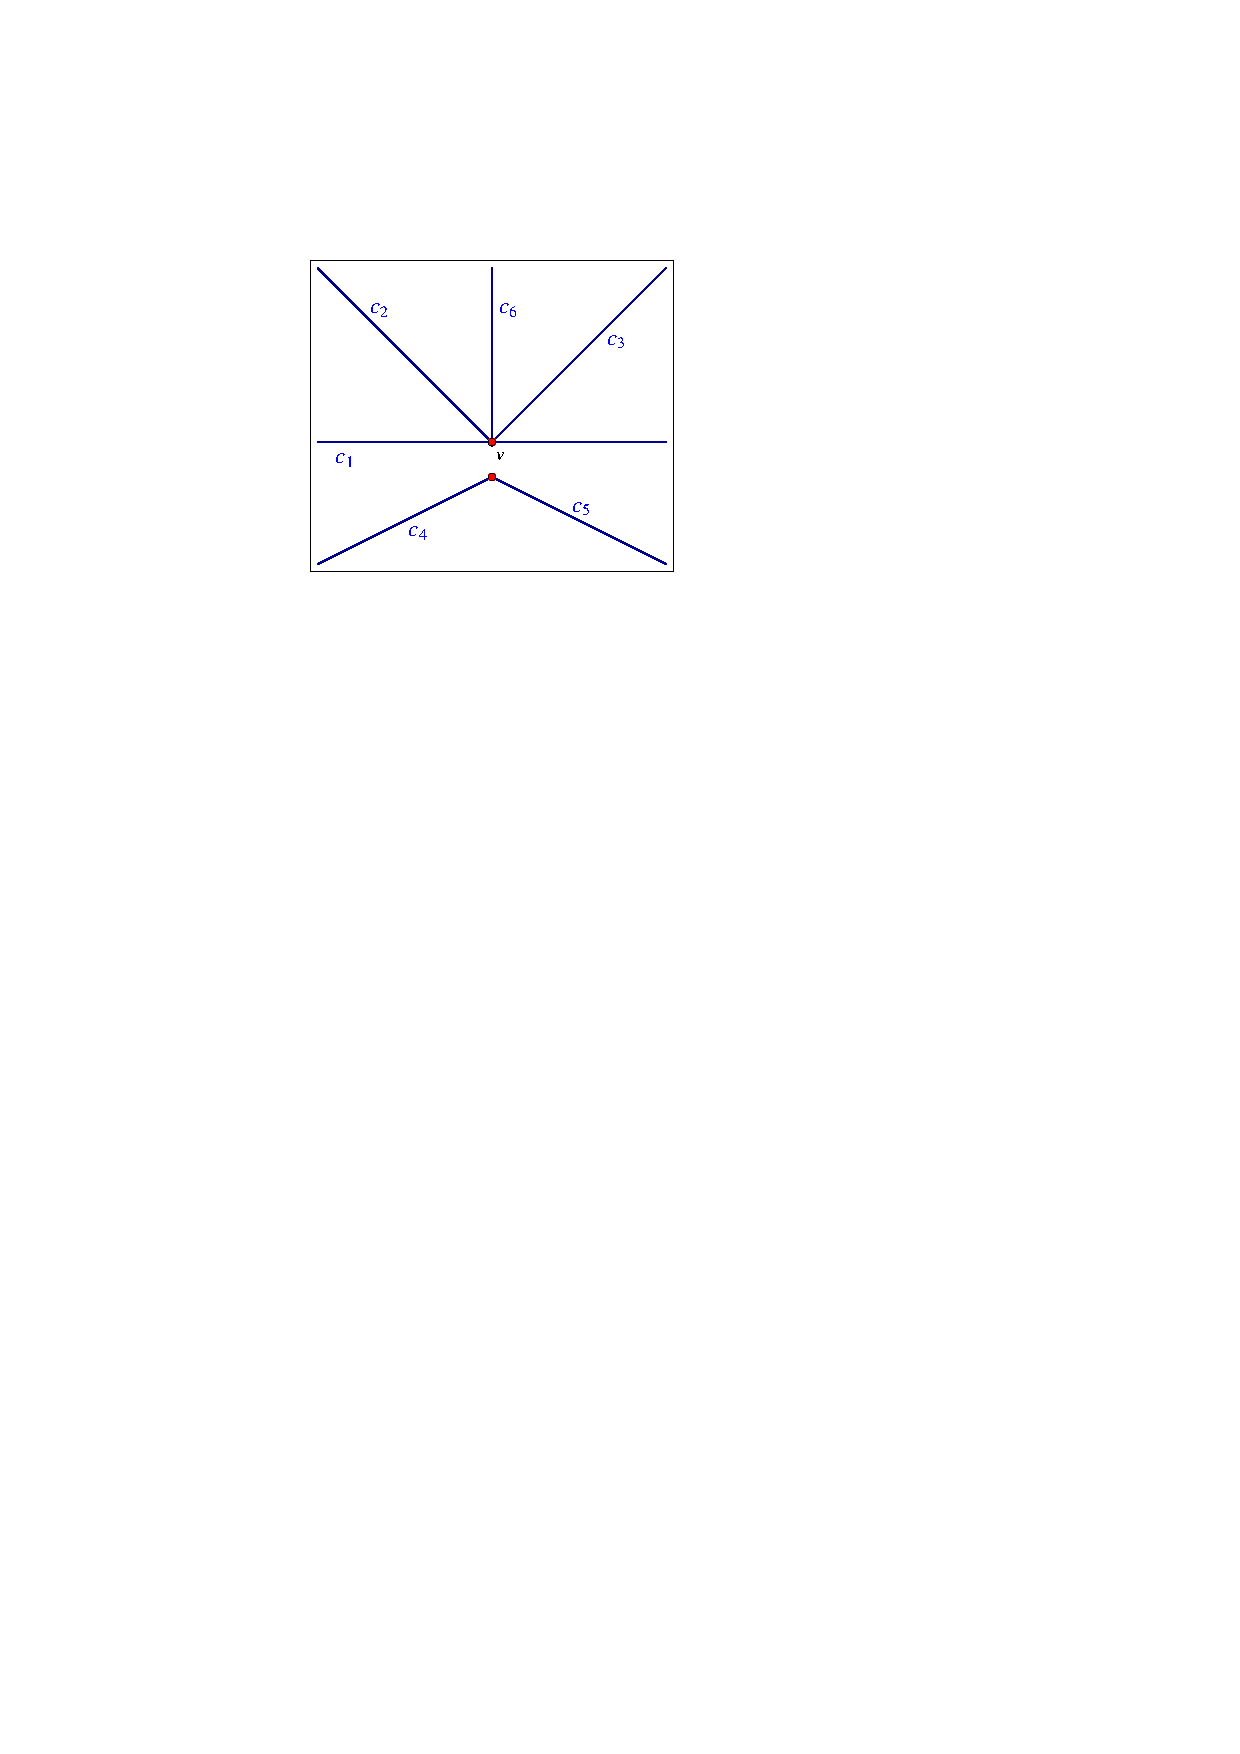
\includegraphics{Arrangement_on_surface_2/fig/ex_unb1}
  \end{center}
\end{ccTexOnly}
\begin{ccHtmlOnly}
  <p><center>
  <img src="./fig/ex_unb1.gif" border=0 alt="Unbounded example 1">
  </center>
\end{ccHtmlOnly}
\caption{An arrangement of unbounded linear objects, as constructed
in \ccc{unbounded_non_intersecting.cpp}.\label{arr_fig:ex_unb1}}
\end{figure}

The following example demonstrates the use of the insertion function
for pairwise interior-disjoint unbounded curves. In this example
we use the traits class \ccc{Arr_linear_traits_2<Kernel>} to
instantiate the \ccc{Arrangement_2} template. This traits class is
capable of representing line segments as well as unbounded linear
curves (namely lines and rays). Observe that objects of the type
\ccc{X_monotone_curve_2} defined by this traits class are
constructible from \ccc{Line_2}, \ccc{Ray_2}, and \ccc{Segment_2}
objects, as defined in the instantiated kernel.

The first three curves are inserted using the special insertion
functions for $x$-monotone curves whose location in the arrangement
is known. Notice that inserting an unbounded curve in the interior
of an unbounded face, or from an existing vertex that represents the
bounded end of the curve, may cause an unbounded face to split (this
is never the case when inserting a bounded curve --- compare with
Section~\ref{arr_sssec:mf_insert_cv}). Then, three additional rays are 
inserted incrementally, using the insertion function for $x$-monotone
curves whose interior is disjoint from all arrangement features.
Finally, the program prints the size of the arrangement (compare to
the illustration in Figure~\ref{arr_fig:ex_unb1}) and the outer
boundaries of its six unbounded faces:

\ccIncludeExampleCode{Arrangement_on_surface_2/unbounded_non_intersecting.cpp}

\subsection{Free Functions\label{arr_ssec:unb_global}}
%---------------------------

In principle, all queries and operations that relate to arrangements
of bounded curves can also be applied to arrangements of unbounded
curves. For example, it is possible to issue point-location and
vertical ray-shooting queries (see also Section~\ref{arr_sec:queries})
on arrangements of lines, where the only restriction is that the query
point has finite coordinates.\footnote{Currently, all point-location
strategies except the trapezoidal RIC point-location strategy are
capable of handling arrangements of unbounded curves.} 

In the following example we show how an arrangement of unbounded lines
is utilized to solve the following problem: Given a set of points, does
the set contain at least three collinear points? In this example a set
of input points is read from a file. The file  \ccc{points.dat} is
used by default. It contains definitions of $100$ points randomly
selected on the grid $[-10000,10000]\times[-10000,10000]$. We
construct an arrangement of the dual lines, where the line $p^{*}$
dual to the point $p = (p_x, p_y)$ is given by the equation
$y = p_x*x - p_y$, and check whether three (or more) of the dual lines
intersect at a common point, by searching for a (dual) vertex, whose
degree is greater than $4$. If such a vertex exists, then there are at
least three dual lines that intersect at a common point, which implies
that there are at least three collinear points.

\ccIncludeExampleCode{Arrangement_on_surface_2/dual_lines.cpp}

Note that there are no three collinear points among the points defined
in the input file \ccc{points.dat}. In the second part of the example
the existence of collinearity is forced and verified as follows. A line
dual to the midpoint of two randomly selected points is introduced,
and inserted into the arrangement. This operation is followed by a
test that verifies that a vertex of degree greater than $4$
exists. This implied that collinearity indeed exists as explained above.

\begin{ccAdvanced}

\subsection{Representation of Unbounded Arrangements\label{arr_ssec:unb_rep}}
%--------------------------------------------

\begin{figure}[t]
\begin{ccTexOnly}
  \begin{center}
  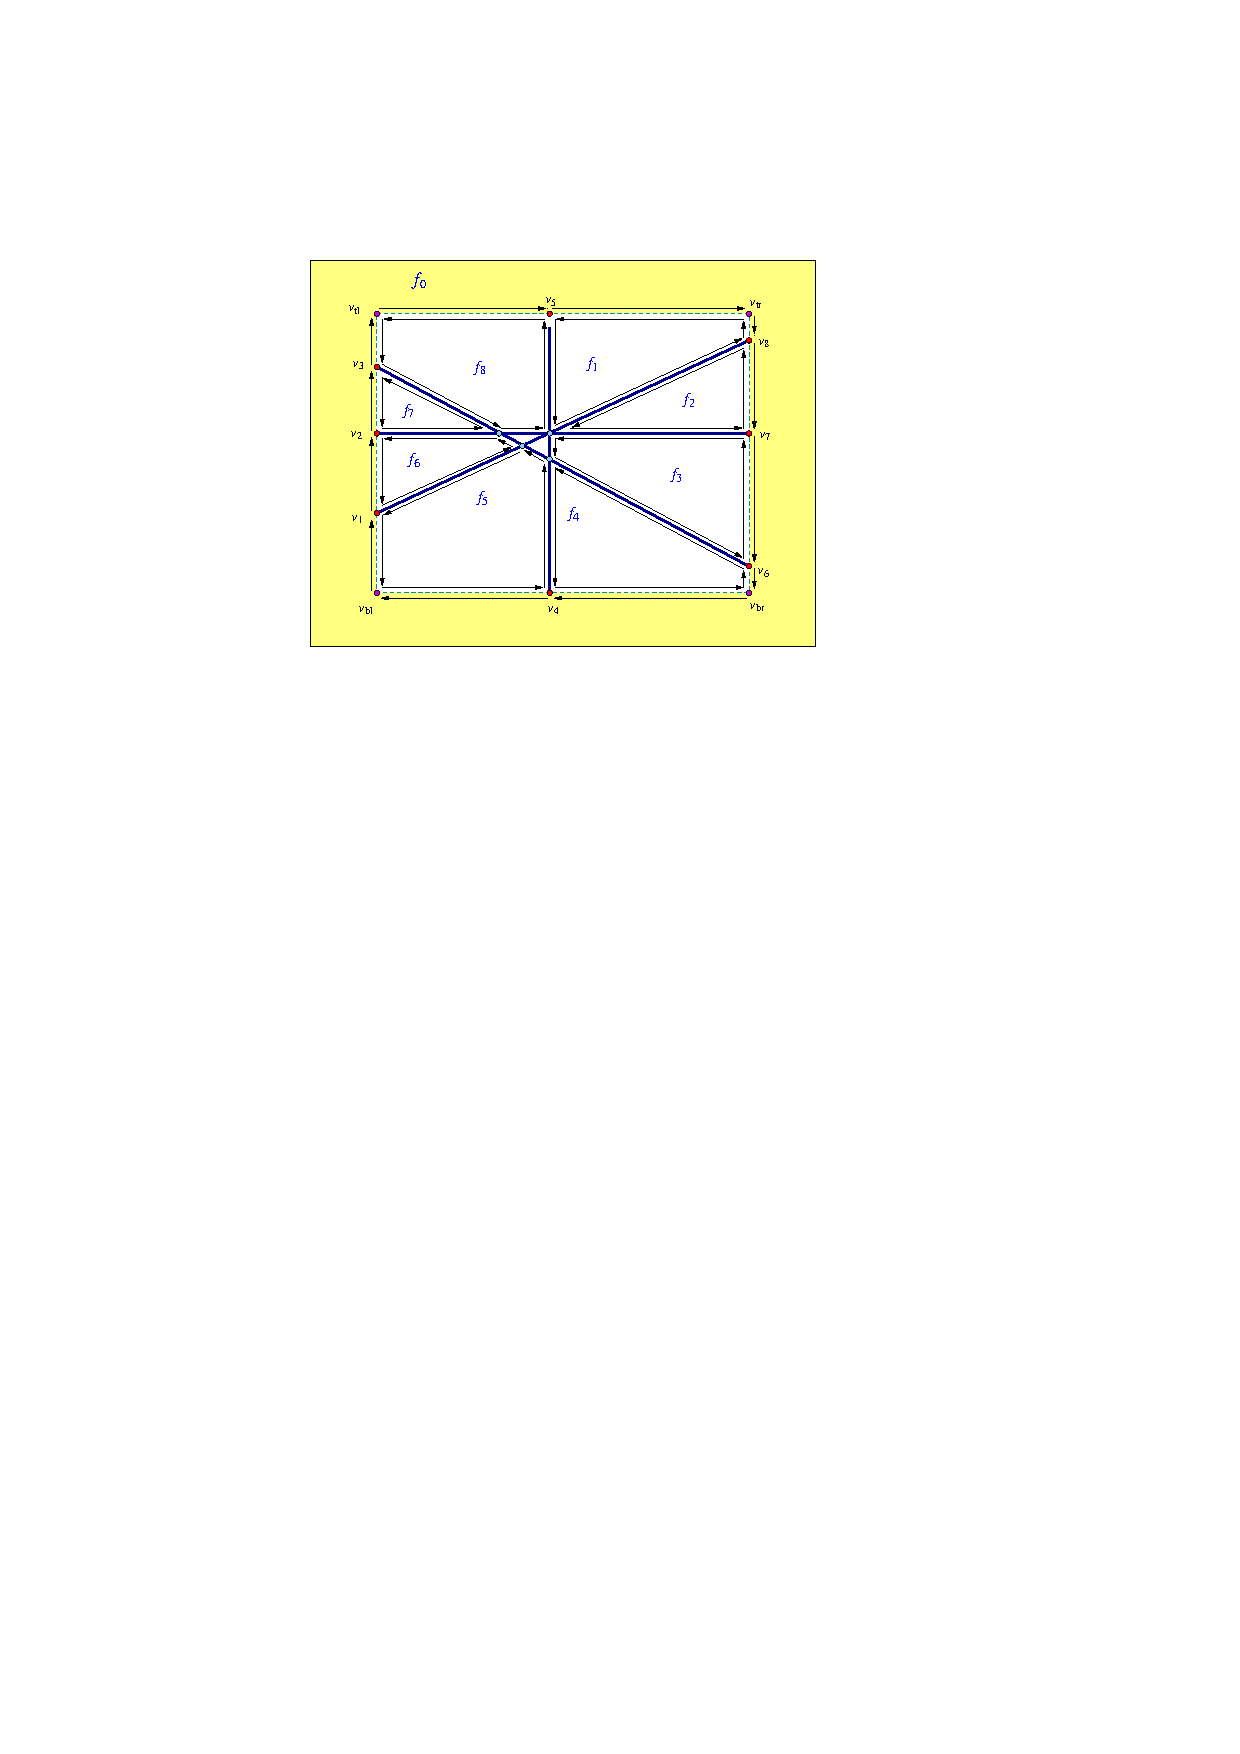
\includegraphics{Arrangement_on_surface_2/fig/unb_dcel}
  \end{center}
\end{ccTexOnly}
\begin{ccHtmlOnly}
  <p><center>
  <img src="./fig/unb_dcel.gif" border=0 alt="Unbounded DCEL">
  </center>
\end{ccHtmlOnly}
\caption{A \dcel\ representing an arrangement of four lines.
Halfedges are drawn as thin arrows. The vertices $v_1, \ldots, v_8$
lie at infinity, and are not associated with valid points. The
halfedges that connect them are fictitious, and are not associated
with concrete curves. The face denoted $f_0$ (lightly shaded)
is the fictitious ``unbounded face'' which lies outside the imaginary
rectangle (dashed) that bounds the actual arrangement. The four
fictitious vertices $v_{\rm bl}, v_{\rm tl}, v_{\rm br}$ and
$v_{\rm tr}$ represent the four corners of the imaginary bounding
rectangle..\label{arr_fig:unb_dcel}}
\end{figure}

Given a set $\calC$ of unbounded curves, a simple approach for
representing the arrangement induced by $\calC$ would be to clip the
unbounded curves using an axis-parallel rectangle that contains all
finite curve endpoints and intersection points between curves in
$\calC$. This process would result in a set $\calC$ of bounded curves
(line segments if $\calC$ contains lines and rays), and it would be
straightforward to compute the arrangement induced by this set.
However, we would like to operate directly on the unbounded curves
without having to preprocess them. Therefore, we use an implicit
bounding rectangle embedded in the \dcel\ structure.
Figure~\ref{arr_fig:unb_dcel} shows the arrangement of four lines
that subdivide the plane into eight unbounded faces and two bounded
ones. Notice that in this case the unbounded faces have outer
boundaries, and the halfedges along these outer CCBs are drawn as 
arrows. The bounding rectangle is drawn with a dashed line. The
vertices $v_1,v_2,\ldots,v_8$, which represent the unbounded ends of 
the four lines, and lie on the bounding rectangle, actually exist at
infinity, and the halfedges connecting them are \emph{fictitious}, and
represent portions of the bounding rectangle. Note that the outer CCBs
of the unbounded faces contain fictitious halfedges. The twins of these
halfedges form together one connected component that corresponds to
the entire imaginary rectangle, which forms a single hole in a face
$\tilde{f}$. We say that $\tilde{f}$ is \emph{fictitious}, as it does
not corresponds to a real two-dimensional cell of the arrangement.

Observe that there are four extra vertices at infinity that do not lie
on any curve; they are denoted as $v_{\rm bl}, v_{\rm tl}, 
v_{\rm br}$, and $v_{\rm tr}$, and represent the bottom-left, top-left,
bottom-right, and top-right corners of the bounding rectangle,
respectively. Similarly, there are fictitious halfedges that lie on
the top, the bottom, the left, or the right edge of the imaginary
bounding rectangle. When the arrangement is empty, there are exactly
four pairs of fictitious halfedges, that divide the plane into two
faces, namely a fictitious face lying outside of the imaginary bounding
rectangle and a single unbounded face bounded by the imaginary
bounding rectangle. 

Summarizing the above, there are four types of arrangement vertices,
which differ from one another by their location on the imaginary
bounding rectangle:
\begin{enumerate}
\item
A ``normal'' vertex, associated with a point in $\real^2$ whose
coordinates are bounded. Such a vertex always lies inside the
bounding rectangle.
\item
A vertex that represent an unbounded end of an $x$-monotone curve
that is defined at $x = -\infty$ or at $x = \infty$. In case of
a horizontal line or a curve with a horizontal asymptote, the
$y$-coordinate of the curve end may be finite (see for example the
vertices $v_2$ and $v_7$ in Figure~\ref{arr_fig:unb_dcel}), but in
general the curve end also goes to $y = \pm\infty$ (see for instance
the vertices $v_1$, $v_3$, $v_6$ and $v_8$ in
Figure~\ref{arr_fig:unb_dcel}). For our convenience, we will always
take a ``tall'' enough bounding rectangle and treat such vertices as
lying on either the left or right rectangle edges (that is, if a curve
is defined at $x = -\infty$, its left end will be represented by
a vertex on the left edge of the bounding rectangle, and if it is
defined at $x = \infty$, its right end will be represented by a
vertex of the right edge).
\item
A vertex that represent the unbounded end of a vertical line or of a
curve with a vertical asymptote (finite $x$-coordinate and an
unbounded $y$-coordinate). Such a vertex always lies on one of the
horizontal edges of the bounding rectangle (either the bottom one if
$y = -\infty$, or the top one if $y = \infty$). The vertices $v_4$ 
and $v_5$ in Figure~\ref{arr_fig:unb_dcel} are of this type.
\item
The fictitious vertices that represent the four corners of the
imaginary bounding rectangle.
\end{enumerate}
A vertex at infinity of types 1--3 above always has
three incident edges: one concrete edge that is associated with an
unbounded portion of an $x$-monotone curve, and two fictitious edges
connecting the vertex to its neighboring vertices at infinity.
Fictitious vertices (of type 4 above) have exactly two incident edges.
See Section~\ref{arr_sec:traits} on how the traits-class interface
helps imposing the fact that we never have more than one curve
incident to any true vertex at infinity.

The nested types defined in the \ccc{Arrangement_2} class support the
following methods, in addition to the ones listed in
Section~\ref{arr_ssec:traverse}:
\begin{itemize}
\item
The \ccc{Vertex} class provides three-valued predicates
\ccc{boundary_in_x()} and \ccc{boundary_in_y()}, which
return \ccc{NO_BOUNDARY} if the vertex has a finite $x$-coordinate (or
$y$-coordinate) and \ccc{MINUS_INFINITY} or \ccc{PLUS_INFINITY} if
the vertex lies at infinity. The Boolean predicate
\ccc{is_at_infinity()} is also supported, where we can access the
point associated with a vertex only if it is not a vertex at infinity
(recall that a vertex at infinity is not associated with a
\ccc{Point_2} object).
%
\item
The nested \ccc{Halfedge} class provides the Boolean predicate
\ccc{is_fictitious()}. The $x$-monotone curve associated with
a halfedge can be accessed by the \ccc{curve()} method only if the
halfedge is not fictitious.
%
\item
The nested \ccc{Face} class provides the Boolean predicate
\ccc{f.is_fictitious()}. The method \ccc{outer_ccb()} has the
precondition that the face is not fictitious. Note that valid
unbounded faces always have valid CCBs (although this CCB may
comprise only fictitious halfedge in case the arrangement contains
only bounded curves).
\end{itemize}

The method \ccc{arr.number_of_edges()} does not count the number of
fictitious edges, (which is always
\ccc{arr.number_of_vertices_at_infinity() + 4}), and the iterators
returned by \ccc{arr.edges_begin()} and \ccc{arr.edges_end()} specify
a range of valid edges. Similarly, \ccc{arr.number_of_faces()} does not
count the fictitious face.
However, the \ccc{Ccb_halfedge_circulator} of the outer boundary of an
unbounded face or the \ccc{Halfegde_around_vertex_circulator} of a vertex
at infinity do traverse fictitious halfedges. For example, it is possible
to traverse the outer boundaries of the unbounded arrangement edges
using the following procedure:
\begin{alltt}
  Arrangement_2::Unbounded_face_const_iterator  fit;
  Arrangement_2::Ccb_halfedge_const_circulator  first, curr;
  Arrangement_2::Halfedge_const_handle          he;
  int                                           k = 1;

  for (fit = arr.unbounded_faces_begin();
       fit != arr.unbounded_faces_end(); ++fit, k++)
  \{
    std::cout << "Unbounded face no. " << k << ": ";
    curr = first = fit->outer_ccb();
    if (! curr->source()->is_at_infinity())
      std::cout << "(" << curr->source()->point() << ")";
    do
    \{
      he = curr;
      if (! he->is_fictitious())
        std::cout << "   [" << he->curve() << "]   ";
      else
        std::cout << "   [ ... ]   ";

      if (! he->target()->is_at_infinity())
        std::cout << "(" << he->target()->point() << ")";

      ++curr;
    \} while (curr != first);
    std::cout << std::endl;
  \}
\end{alltt}

\end{ccAdvanced}
